% !TeX root = ../document.tex

\section{Introduction}

The following chapter describes interpolation in general with regard to the most frequently used methods. We will give an introduction to the background of each method, their suitability/advantages and disadvantages as well as examples of application in other studies. Furthermore, we present possibilities of carrying out interpolation analysis and an overview of which methods are supported by a variety of FOSSGIS tools.


\subsection{Statistical and Deterministic methods?}

A deterministic method always generates the exact same output for a given input. Thus, leading to reproducible results, whereas a statistical method might not generate the same results.
% TODO: Should we keep this?

\subsection{What is spatial interpolation?}

Spatial interpolation is the calculation of nearby and unknown values ​​on the basis of neighboring known values. \cite{gitta_raumliche_2016} Interpolation methods are often used for analyzing spatial and spatio-temporal distributions of physical but also socioeconomic phenomena. These phenomena can be approximated by certain functions, which are location dependent within space \cite{mitas_spatial_1999}. Interpolation is thus very useful for estimating or predicting missing geographic point data, such as elevation, rainfall, chemical concentrations, noise levels etc. \cite{samanta_interpolation_2012}. Calculating these unknown values is done via a series of different methods, where the methods themselves again depend on the research question and the data present. In this study we will be focusing on temperature data only and give a short overview of similar studies and their choice of method.

\subsection{The diversity of methods}

In this chapter, we will give a short introduction to the various methods, starting off with a general possibility of classification – a schematic overview. According to \fullcite{hofstra_comparison_2008} the choice of method, when interpolating climate-related data, depends primarily on the different variables, station densities and climate regimes. It is rather difficult to find a single method which fulfills all requirements. Thus, the goal is to give an overview of different (and widely used) interpolation methods (mostly in the context of climate-related research) and present some advantages and disadvantages of each method as well as give some examples of their application.

\subsubsection{Interpolation: Schematic overview}

Generally, there is a difference between global and local interpolation, whereas global interpolation is not suitable for determining values ​​that are as exact as possible, but for assessing rough global spatial structures. \cite{gitta_raumliche_2016}
Interpolation methods are also distinguishable in exact and non-exact or gradual and abrupt interpolation (see figure \ref{fig:exact_non_exact_interploation}). On the left, the generated surface, which stands for the resulting interpolation, fits exactly to the data points, although the surface has abrupt  \ldq{}steps\rdq{} (the used method here is the Natural Neighbor interpolation). Adjusting the interpolation surface results in a smoother surface, as seen in figure \ref{fig:exact_non_exact_interploation} on the right.
% TODO: zweimal the used method...
The used method, the inverse distance weighting (IDW), does not follow the high and low data points exactly, which is why a \ldq{}moving average\rdq{} or \ldq{}smoothing\rdq{} of the data occurs. In the end, the choice depends on whether  \ldq{}[...] we need the interpolated surface to exactly pass through the data points or we require a surface which simply represents the general trend\rdq{}. %TODO: cite (Wyatt, o. J.). 



\begin{figure}
	\begin{minipage}[b]{.48\linewidth}
		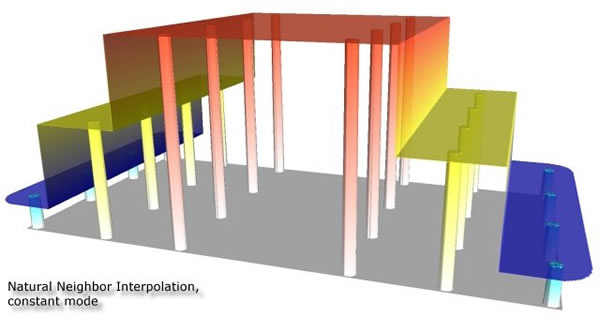
\includegraphics[width=\linewidth]{images/exakte_interpolation.jpg}
	\end{minipage}
	\hfill
	\begin{minipage}[b]{.48\linewidth}
		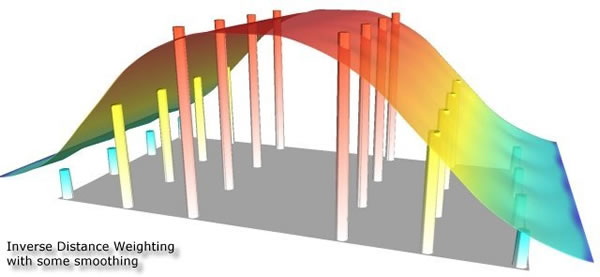
\includegraphics[width=\linewidth]{images/nicht_exakte_interpolation.jpg}
	\end{minipage}
	\label{fig:exact_non_exact_interploation}
	\caption{Different interpolation surfaces due to exact (left) and non-exact (right) interpolation\cite{gitta_raumliche_2016}}
\end{figure}

And finally, we can differentiate between deterministic and stochastic methods.\cite{gitta_raumliche_2016}
Deterministic methods encompass for example \ldq{}TIN\rdq{}, \ldq{}IDW\rdq{} or \ldq{}Spline\rdq{}. \cite{wasser_going_2020} Deterministic interpolation techniques are generally based on precisely predictable (= deterministic) spatial relationships, whereas stochastic, or also called probabilistic or geostatistical) methods, make use of underlying statistical properties of the point data. Latter requires advanced knowledge, which is why will focus primarily on deterministic methods. One of the most prominent and important stochastic methods is Kriging.

In regard to suitability, we refer to figure \ref{fig:interpolation_methods_strengths}, which gives a good overview for several of the methods and their advantages and disadvantages. As the choice of method is, as already stated, dependent on the question one poses and the data available, no general statement can be given. 


\begin{figure}
	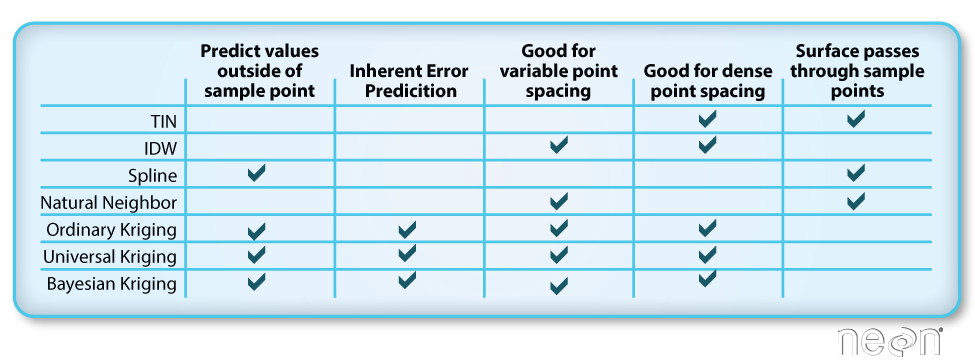
\includegraphics[width=\linewidth]{images/interpolation_methods_strengths.png}
	\label{fig:interpolation_methods_strengths}
	\caption{Strengths of interpolation methods \cite{wasser_going_2020}}
\end{figure}

